%% Section 7: Robustness and Sensitivity Analysis
%% STATUS: STUB — figure placeholder and table shell present.
%% See artifacts/revision2/SIGMETRICS_OUTLINE.md §7 for planned content (~2 pages).

\section{Robustness and Sensitivity Analysis}
\label{sec:robustness}

\subsection{E1: Cabinet-Envelope Scale Sensitivity}
% source: artifacts/revision2/sensitivity_cabinet_scale.json
%   5 scale factors [0.90, 0.95, 1.00, 1.05, 1.10], FP_vs_Random at r=1.25
%   0.90: +0.814 pp [+0.002, +2.381]  18/6/1
%   0.95: +2.977 pp [+0.547, +4.278]  21/4/0
%   1.00: +6.706 pp [+3.920, +8.725]  22/1/2 (primary)
%   1.05: +4.404 pp [+3.202, +5.536]  20/3/2
%   1.10: +4.687 pp [+0.871, +5.330]  20/2/3
%   Result: sign positive at all 5 scale factors
% Note: at scale=0.90, CI barely clears zero ([+0.002, +2.381]).
% Post-exposure disclosure applies (see §5).

\subsection{E2: Beta Sensitivity}
% source: artifacts/revision2/sensitivity_loo_beta.json
%   6 beta values: primary (1.114), frozen (1.125), prospective (0.96),
%                  jackknife (1.083), CF-P5 (1.066), CF-P95 (1.169)
%   All medians positive; no sign reversal. Result: stable (no sign reversal).
% Post-exposure disclosure applies (see §5).

\begin{table}[t]
\caption{E1/E2 sensitivity analysis results. Panel A (E1): FP vs.\ Random at
$r=1.25$ across five cabinet-envelope scale factors; sign positive at all five. Panel B (E2):
across six pre-specified beta estimator variants; no sign reversal. Post-exposure
disclosure: E1/E2 were prespecified at commit 5733b73 but executed after primary
results were exposed; design was not changed.}
\label{tab:sensitivity}
\centering
\begin{tabular}{lrrr}
\toprule
& n\,/\,I\,/\,B & Median $\delta_{\mathrm{lo}}$ & Bootstrap 95\%~CI \\
\midrule
\multicolumn{4}{l}{\textit{Panel A --- E1: Cabinet scale}} \\
Scale 0.90 & 18\,/\,6\,/\,1 & $+0.81$ pp & $[{+}0.002, {+}2.38]$ \\
Scale 0.95 & 21\,/\,4\,/\,0 & $+2.98$ pp & $[{+}0.55, {+}4.28]$ \\
\textbf{Scale 1.00 (primary)} & \textbf{22\,/\,1\,/\,2} & $+6.71$ pp & $[{+}3.92, {+}8.72]$ \\
Scale 1.05 & 20\,/\,3\,/\,2 & $+4.40$ pp & $[{+}3.20, {+}5.54]$ \\
Scale 1.10 & 20\,/\,2\,/\,3 & $+4.69$ pp & $[{+}0.87, {+}5.33]$ \\
\midrule
\multicolumn{4}{l}{\textit{Panel B --- E2: Beta value}} \\
\textbf{Primary (LOO CF, 1.114)} & \textbf{22\,/\,1\,/\,2} & $+6.71$ pp & $[{+}3.92, {+}8.72]$ \\
Frozen (1.125)        & 22\,/\,1\,/\,2 & $+6.48$ pp & $[{+}3.92, {+}8.72]$ \\
2025 in-sample (0.960) & 22\,/\,1\,/\,2 & $+6.67$ pp & $[{+}2.08, {+}7.04]$ \\
Jackknife (1.083)     & 22\,/\,1\,/\,2 & $+5.59$ pp & $[{+}3.92, {+}8.72]$ \\
CF P5 (1.066)         & 21\,/\,2\,/\,2 & $+6.42$ pp & $[{+}3.20, {+}8.72]$ \\
CF P95 (1.169)        & 22\,/\,1\,/\,2 & $+5.35$ pp & $[{+}2.16, {+}8.72]$ \\
\bottomrule
\end{tabular}
% source Panel A: artifacts/revision2/sensitivity_cabinet_scale.json
% source Panel B: artifacts/revision2/sensitivity_loo_beta.json
\end{table}

% Figure 5: Robustness panels (E1 + E2)
\begin{figure}[t]
\centering
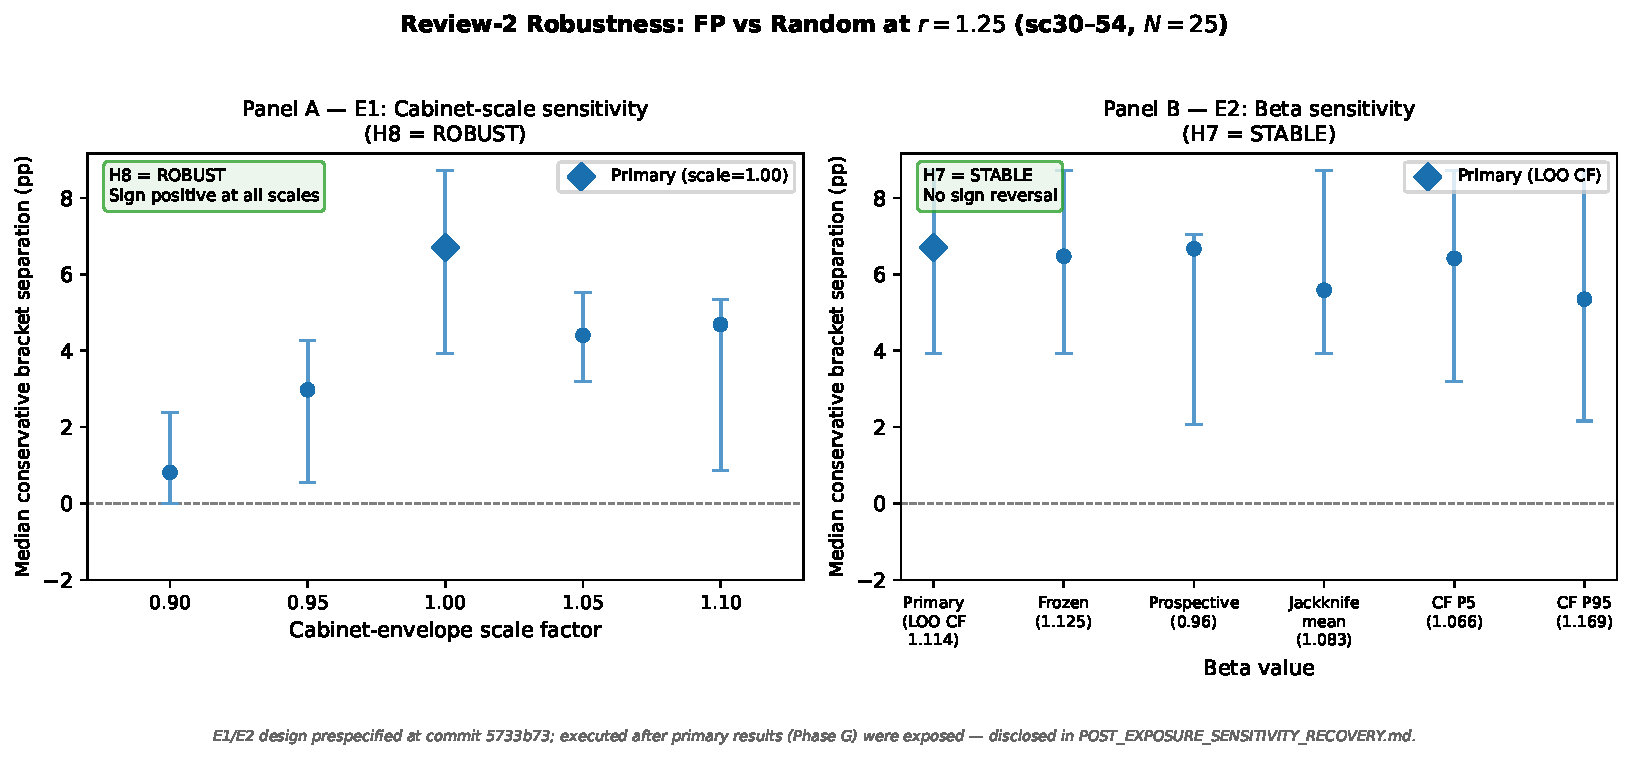
\includegraphics[width=\textwidth]{fig_r2_robustness}
% source: artifacts/revision2/figures/fig_r2_robustness.pdf (300 dpi)
% generation: artifacts/revision2/figures/fig_r2_robustness.py
\caption{Robustness analysis. Panel A (E1): FP vs.\ Random median
$\delta_{\mathrm{lo}}$ (pp) across five cabinet-envelope scale factors
$[0.90, 1.10]$; sign positive at all scales; barely clearing
zero at $-10\%$). Panel B (E2): across six pre-specified beta estimator
variants; no sign reversal. Primary value highlighted (diamond).
Error bars: bootstrap 95\%~CI.}
\label{fig:robustness}
\end{figure}
